\documentclass[final,t]{beamer}
\usepackage[size=a0,orientation=portrait,scale=1.15]{beamerposter}

\usepackage[utf8]{inputenc}
\usepackage[T1]{fontenc}
\usepackage[english]{babel}
\usepackage{graphicx}
\usepackage{amsmath,amssymb}
\usepackage{tikz}
\usetikzlibrary{positioning,arrows.meta,shapes.geometric,backgrounds,calc,shadows}
\usepackage{booktabs}
\usepackage{tabularx}
\usepackage{colortbl}
\usepackage[sfdefault]{roboto}                 % display sans — pdflatex compatible

% --- PWr colour scheme + accents ---
\definecolor{pwrred}{HTML}{9A342D}
\definecolor{pwrbeige}{HTML}{F0D0A1}
\definecolor{pwrdark}{HTML}{5C1C18}
\definecolor{cardgrey}{HTML}{F4F2EE}
\definecolor{accentblue}{HTML}{2B6E8C}
\definecolor{neutralgrey}{HTML}{6B6B6B}
\definecolor{lightgrey}{HTML}{B5B5B5}

\setbeamercolor{background canvas}{bg=white}
\setbeamercolor{normal text}{fg=black,bg=white}
\setbeamertemplate{navigation symbols}{}
\setbeamertemplate{headline}{}
\setbeamertemplate{footline}{}

\title{}
\begin{document}
\begin{frame}[t,fragile]
\vspace*{-2cm}
\begin{tikzpicture}[remember picture, overlay]

%==========================================================
% HEADER — top white strip with logo + ICAISC, then red title bar
%==========================================================

% White strip: 0-6 cm from top, with logo on left and ICAISC banner on right
\fill[white] (current page.north west) rectangle ([yshift=-6cm]current page.north east);

\node[anchor=north west, inner sep=0pt]
  at ([xshift=2.5cm,yshift=-1.3cm]current page.north west)
  {
\includegraphics[height=3.4cm]{logo_PWR.png}};

\node[anchor=north east, inner sep=0pt, align=right, text=pwrdark]
  at ([xshift=-2.5cm,yshift=-1.5cm]current page.north east)
  {%
  \fontsize{34}{38}\selectfont\bfseries
  ICAISC 2026
  \\[0.2em]
  \fontsize{22}{26}\selectfont\mdseries
  Zakopane, Poland
  };

% Red title bar: 6-19 cm from top
\fill[pwrred] ([yshift=-6cm]current page.north west)
              rectangle ([yshift=-19cm]current page.north east);

\node[anchor=north, text=pwrbeige, align=center, inner sep=0pt,
      yshift=-7cm, text width=0.92\paperwidth]
  at (current page.north)
  {%
  \fontsize{90}{104}\selectfont\bfseries
  The Fibonacci Neighborhood\\[0.1em]
  \fontsize{52}{62}\selectfont\mdseries
  beats Adjacent and Dynasearch from \textit{n}\,=\,200
  };

\node[anchor=north, text=pwrbeige, align=center, yshift=-16.5cm]
  at (current page.north)
  {%
  \fontsize{30}{36}\selectfont
  Remigiusz Wojew\'odzki~~\textbullet~~Wojciech Bo\.zejko
  \hspace{1.5em}|\hspace{1.5em}
  Wroc\l{}aw University of Science and Technology
  };

%==========================================================
% HERO BAND — KEY RESULT IN BIG NUMBERS
%==========================================================
\fill[pwrbeige] ([yshift=-19cm]current page.north west)
                rectangle ([yshift=-32cm]current page.north east);

\node[anchor=north, yshift=-19.8cm] at (current page.north)
  {\fontsize{30}{34}\selectfont\bfseries\color{pwrdark}
   At $n=200$, $m=20$, $tl=5\,\text{s}$, Tabu Search:};

\node[anchor=center, yshift=-26.4cm] at (current page.north)
  {\begin{tikzpicture}
    % three big numbers in cards
    \node[draw=pwrred, fill=white, line width=2pt, rounded corners=8pt,
          minimum width=14cm, minimum height=8cm, align=center, drop shadow] (fib) at (0,0)
       {\fontsize{96}{110}\selectfont\bfseries\color{pwrred} 12.71\%\\[0.3em]
        \fontsize{30}{34}\selectfont\bfseries Fibonacci\\
        \fontsize{22}{26}\selectfont\mdseries\color{neutralgrey}\itshape this work};
    \node[draw=lightgrey, fill=cardgrey, line width=1.5pt, rounded corners=8pt,
          minimum width=12cm, minimum height=7cm, align=center, right=2cm of fib]
       {\fontsize{72}{84}\selectfont\bfseries\color{neutralgrey} 13.20\%\\[0.2em]
        \fontsize{26}{30}\selectfont\bfseries Dynasearch\\
        \fontsize{20}{24}\selectfont\mdseries\color{neutralgrey} segment swaps, $O(mn^3)$};
    \node[draw=lightgrey, fill=cardgrey, line width=1.5pt, rounded corners=8pt,
          minimum width=12cm, minimum height=7cm, align=center, left=2cm of fib]
       {\fontsize{72}{84}\selectfont\bfseries\color{neutralgrey} 13.19\%\\[0.2em]
        \fontsize{26}{30}\selectfont\bfseries Adjacent\\
        \fontsize{20}{24}\selectfont\mdseries\color{neutralgrey} single swap, $O(mn)$};
   \end{tikzpicture}};

\node[anchor=north, yshift=-30.5cm, text=pwrdark, align=center] at (current page.north)
  {\fontsize{26}{30}\selectfont
   \textbf{0.48\,pp better than Adjacent, 0.49\,pp better than Dynasearch}
   ~~ at quadratic per-iteration cost};

\end{tikzpicture}

%==========================================================
% MAIN CONTENT (below the hero band)
%==========================================================
\vspace{34cm}

\begin{columns}[T,totalwidth=\textwidth]

%--------------------------------------------------
% LEFT COLUMN — METHOD
%--------------------------------------------------
\begin{column}{0.48\textwidth}

{\fontsize{42}{50}\selectfont\bfseries\color{pwrred} The Fibonacci move}\\[0.6em]
{\color{pwrred}\rule{\textwidth}{3pt}}\\[0.8em]

{\fontsize{28}{34}\selectfont
A composite move is a subset $S \subseteq \{1,\dots,n{-}1\}$ of
adjacent-swap positions with \textbf{no two consecutive selected}:
\[
\fontsize{34}{40}\selectfont
i \in S \;\Longrightarrow\; i+1 \notin S.
\]
All selected swaps $\pi_i \leftrightarrow \pi_{i+1}$ are applied
\textbf{simultaneously}.
\par}

\vspace{1em}
\begin{center}
\begin{tikzpicture}[scale=1.6]
  \foreach \x in {0,1,2,3,4,5,6,7} \fill[pwrdark] (\x,0) circle (8pt) node[below=14pt, font=\Large] {\x};
  \draw[ultra thick, pwrred] (0,0) to[bend left=80] (1,0);
  \draw[ultra thick, pwrred] (2,0) to[bend left=80] (3,0);
  \draw[ultra thick, pwrred] (5,0) to[bend left=80] (6,0);
  \node[above=10pt, pwrred, font=\Large\bfseries] at (0.5,0.55) {swap};
  \node[above=10pt, pwrred, font=\Large\bfseries] at (2.5,0.55) {swap};
  \node[above=10pt, pwrred, font=\Large\bfseries] at (5.5,0.55) {swap};
\end{tikzpicture}
\end{center}

\vspace{0.5em}
{\fontsize{28}{34}\selectfont
\textbf{Why "Fibonacci"?}\ The number of valid subsets in a permutation
of length $n$ equals the Fibonacci number $F_{n+1}$.
\par}

\vspace{1.6em}
{\fontsize{42}{50}\selectfont\bfseries\color{pwrred} Algorithm — one DP pass}\\[0.6em]
{\color{pwrred}\rule{\textwidth}{3pt}}\\[0.8em]

\begin{center}
\begin{tikzpicture}[node distance=1.2cm, font=\Large]
  \node[draw, fill=cardgrey, rounded corners, minimum width=10cm, minimum height=2cm, align=center]
       (s1) {\textbf{1.} Recompute $C_{\max}(\pi^{(i)})$ for all $i$ \\[-2pt] \footnotesize\color{neutralgrey}$O(mn)$ each};
  \node[draw, fill=pwrbeige, rounded corners, minimum width=10cm, minimum height=2cm, align=center, below=of s1]
       (s2) {\textbf{2.} DP picks optimal non-overlapping subset \\[-2pt] \footnotesize\color{neutralgrey}$\mathrm{dp}[i] = \min(\mathrm{dp}[i+1],\, \Delta_i + \mathrm{dp}[i+2])$};
  \node[draw, fill=cardgrey, rounded corners, minimum width=10cm, minimum height=2cm, align=center, below=of s2]
       (s3) {\textbf{3.} Apply all selected swaps at once};
  \draw[->, ultra thick, pwrred] (s1) -- (s2);
  \draw[->, ultra thick, pwrred] (s2) -- (s3);
\end{tikzpicture}
\end{center}

\vspace{1.2em}
\begin{center}
{\fontsize{26}{30}\selectfont
\begin{tabular}{lcc}
\toprule
\textbf{Neighborhood} & \textbf{Candidates} & \textbf{Per-iter cost} \\
\midrule
Adjacent              & $n-1$                & $O(mn)$        \\
\rowcolor{pwrbeige!50}
\textbf{Fibonacci}    & $n-1\ \text{ + DP}$  & \boldmath$O(mn^2)$ \\
Dynasearch (rec.)     & $O(n^2)$ segments    & $O(mn^3)$      \\
\bottomrule
\end{tabular}
}
\end{center}

\vspace{0.4em}
\begin{center}
\colorbox{pwrred!10}{\parbox{0.92\textwidth}{\centering
\fontsize{28}{34}\selectfont\color{pwrdark}
$F_{n+1}$ valid moves explored at \textbf{quadratic} cost — \\
the sweet spot between cheap (Adjacent) and deep (Dynasearch).
}}
\end{center}

\end{column}

%--------------------------------------------------
% RIGHT COLUMN — RESULTS
%--------------------------------------------------
\begin{column}{0.48\textwidth}

{\fontsize{42}{50}\selectfont\bfseries\color{pwrred} Where Fibonacci wins}\\[0.6em]
{\color{pwrred}\rule{\textwidth}{3pt}}\\[0.6em]

\begin{center}
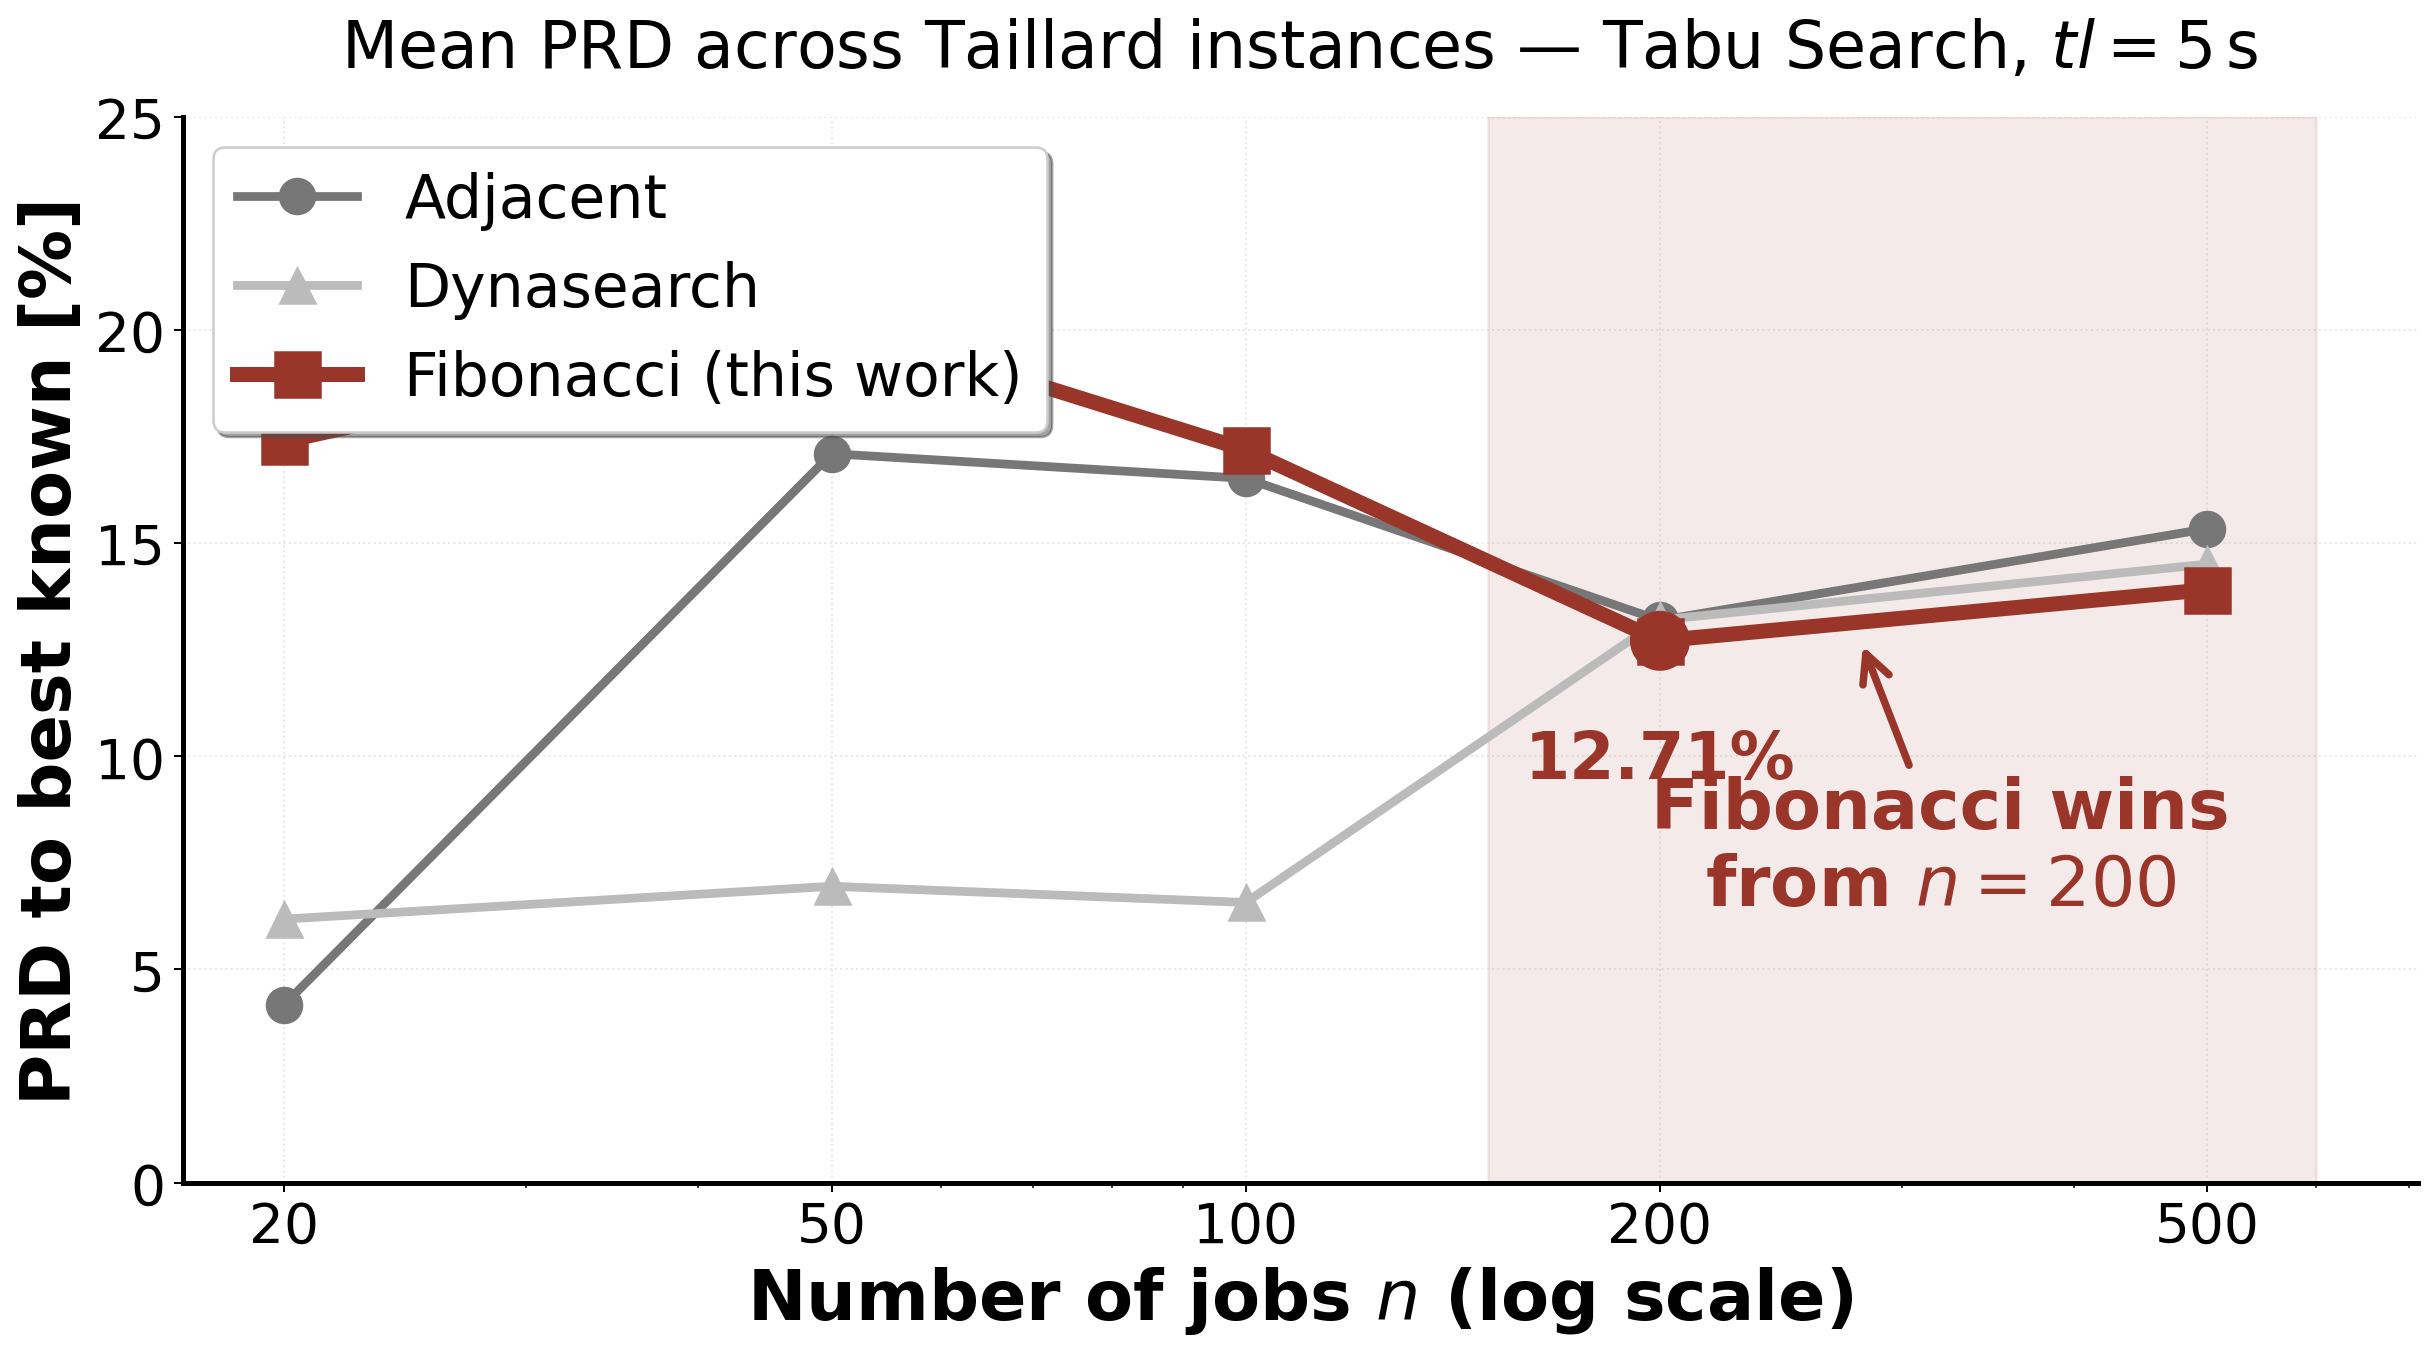
\includegraphics[width=\textwidth]{img/hero_crossover.png}
\end{center}

\vspace{0.5em}
{\fontsize{26}{32}\selectfont
\textbf{Crossover at $n=200$.}\ Below $n=100$ Dynasearch's deep
moves dominate. From $n=200$ Dynasearch's $O(mn^3)$ cost makes it
unable to finish a single iteration within the budget — Fibonacci's
cheaper compound move pulls ahead and stays competitive at $n=500$.
\par}

\vspace{1.5em}
{\fontsize{42}{50}\selectfont\bfseries\color{pwrred} Convergence \,—\, $tl = 1\,$s}\\[0.6em]
{\color{pwrred}\rule{\textwidth}{3pt}}\\[0.8em]

\begin{center}
\begin{tikzpicture}
  \node[anchor=south] (a) at (0,0) {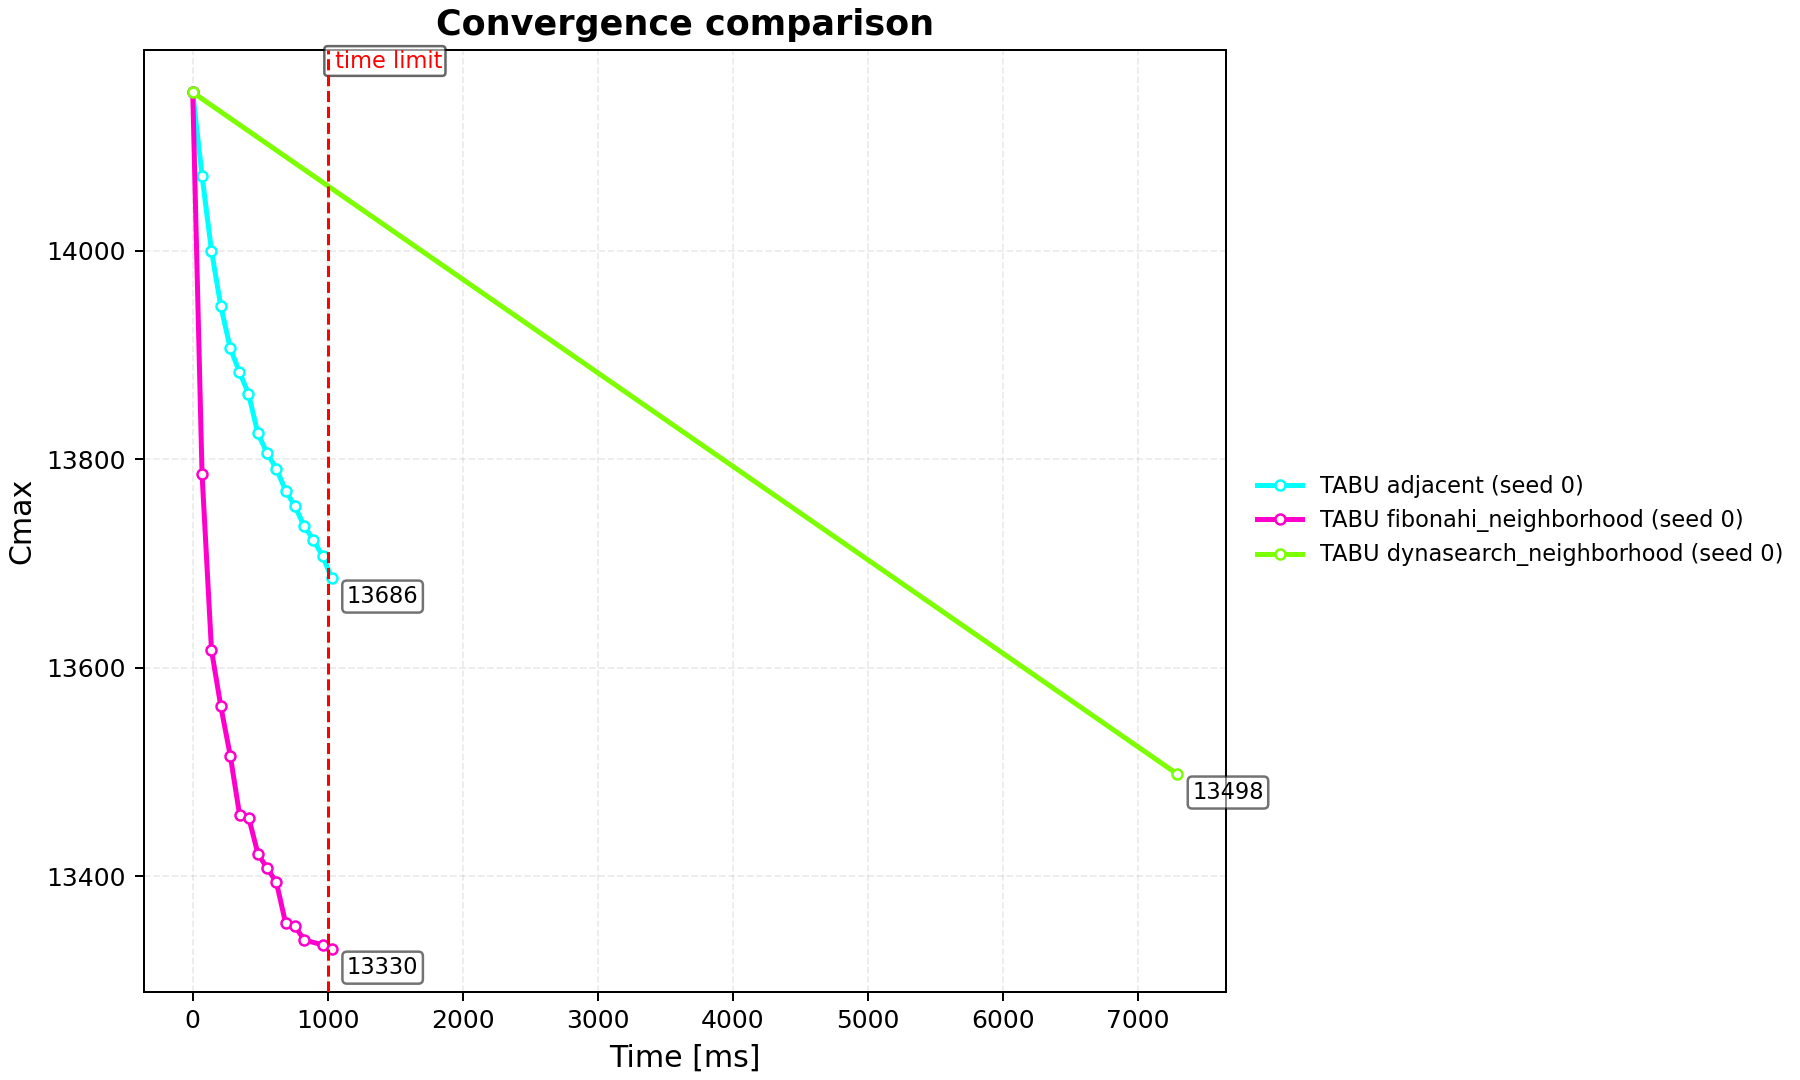
\includegraphics[width=0.49\textwidth]{img/conv_n200.png}};
  \node[anchor=south] (b) at ($(a.south east) + (1cm,0)$) {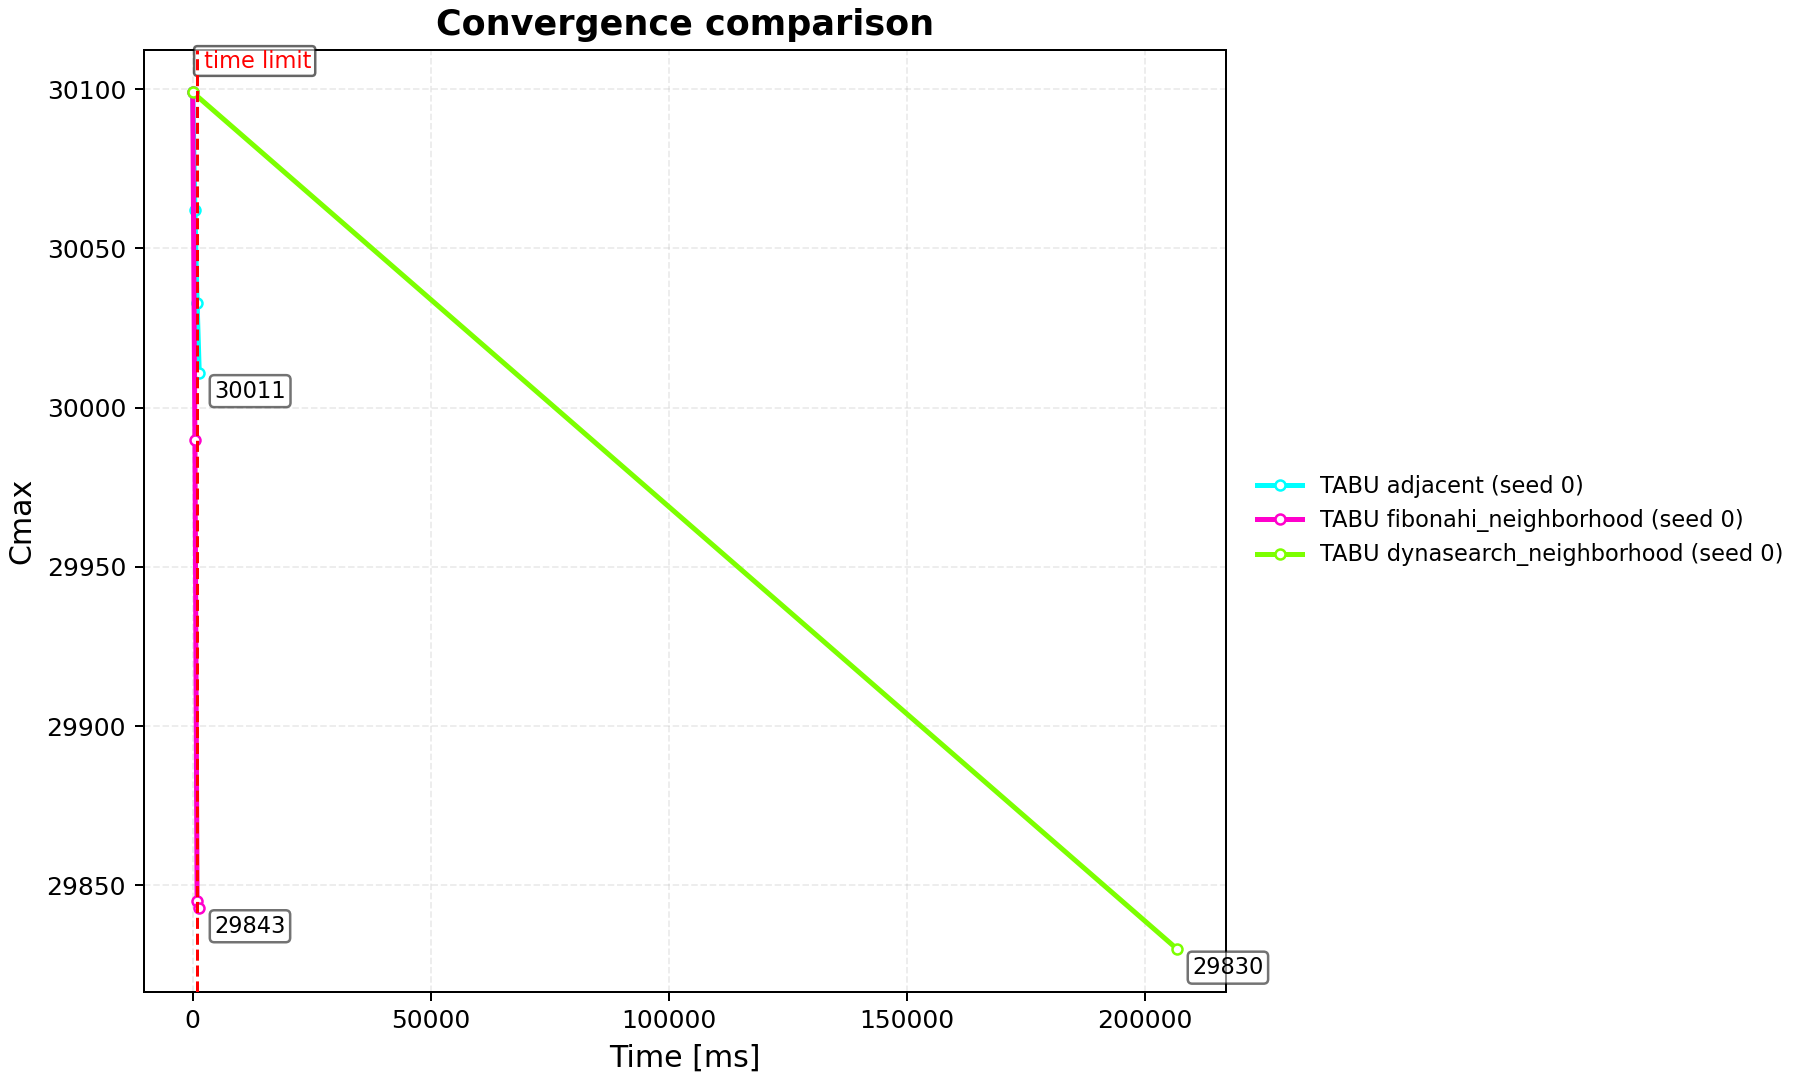
\includegraphics[width=0.49\textwidth]{img/conv_n500.png}};
  \node[below=4pt of a, font=\Large\bfseries\color{pwrdark}] {tai200\_20};
  \node[below=4pt of b, font=\Large\bfseries\color{pwrdark}] {tai500\_20};
\end{tikzpicture}
\end{center}

\vspace{0.8em}
{\fontsize{26}{32}\selectfont
Fibonacci (\textcolor{pwrred}{\textbf{magenta}}) drops $C_{\max}$ in the
first $\sim 100$\,ms. Dynasearch (orange) barely finishes \emph{one}
iteration within the budget.\par}

\vspace{1.6em}
{\fontsize{42}{50}\selectfont\bfseries\color{pwrred} Take-aways}\\[0.6em]
{\color{pwrred}\rule{\textwidth}{3pt}}\\[0.8em]

\begin{center}
\begin{tikzpicture}[node distance=0.6cm, font=\Large]
  \node[draw=pwrred, line width=2pt, fill=white, rounded corners,
        minimum width=0.92\textwidth, minimum height=2.4cm, align=left,
        text width=0.86\textwidth] (t1)
        {\textbf{\large\color{pwrred} Default for $n \geq 200$:}\ Fibonacci, period.};
  \node[draw=pwrred, line width=2pt, fill=white, rounded corners,
        minimum width=0.92\textwidth, minimum height=2.4cm, align=left,
        text width=0.86\textwidth, below=of t1] (t2)
        {\textbf{\large\color{pwrred} SA reheating} rescues the composite move from plateaus once all $\Delta_i \geq 0$.};
  \node[draw=pwrred, line width=2pt, fill=white, rounded corners,
        minimum width=0.92\textwidth, minimum height=2.4cm, align=left,
        text width=0.86\textwidth, below=of t2] (t3)
        {\textbf{\large\color{pwrred} Dynasearch at $n=500$} can need $200\times$ the budget for a single iteration — skip it under tight $tl$.};
\end{tikzpicture}
\end{center}

\end{column}
\end{columns}

%==========================================================
% FOOTER BAND
%==========================================================
\vspace{1.5em}
{\color{pwrred}\rule{\textwidth}{3pt}}\\[0.5em]
\begin{minipage}{0.66\textwidth}
{\fontsize{22}{26}\selectfont
\textbf{Setup.}\ Taillard, $n \in \{20,50,100,200,500\}$, $m \in \{5,10,20\}$.\ \
TS $\tau_{\text{tabu}}{=}10$; SA $T_0{=}1000$, $\alpha{=}0.95$, reheat $r{=}1.5$, stagnation 500\,ms.\ \
Platform: MacBook Pro M4 Pro, Python 3.11.
\par}
\end{minipage}\hfill
\begin{minipage}{0.30\textwidth}
\raggedleft
{\fontsize{22}{26}\selectfont
\textbf{Full paper:}\ ICAISC 2026, Springer LNCS.\\
\textbf{Code:}\ \texttt{github.com/RemigiuszWoj/PhD}
\par}
\end{minipage}

\end{frame}
\end{document}
